%	% ****** Start of file MolecularSpinFlipLoss.tex ******
%
%
%

\documentclass[%
 reprint,
%superscriptaddress,
%groupedaddress,
%unsortedaddress,
%runinaddress,
%frontmatterverbose,
%preprint,
%showpacs,preprintnumbers,
%nofootinbib,
%nobibnotes,
%bibnotes,
 amsmath,amssymb,
 aps,
prl,
%pra,
%prb,
%rmp,
%prstab,
%prstper,
%floatfix,
]{revtex4-1}

\usepackage{graphicx}% Include figure files
\usepackage{dcolumn}% Align table columns on decimal point
\usepackage{bm}% bold math
\usepackage[hidelinks]{hyperref}% add hypertext capabilities
%\usepackage[mathlines]{lineno}% Enable numbering of text and display math
%\linenumbers\relax % Commence numbering lines
\usepackage{textcomp}

\usepackage{color}
\newcommand{\red}[1]{{\color{black} #1}}

% Define new commands for common phrases and standardized typesetting
\newcommand{\exmple}{This is an Example.}



\begin{document}

\title{New Strategy for Stark Deceleration}%

\author{David Reens}
\thanks{dave.reens@colorado.edu.}
\altaffiliation{Present Address: Lincoln Laboratory, Massachusetts Institute of Technology, Lexington, Massachusetts 02420, USA}


\author{Hao Wu}
\altaffiliation{Present Address: Department of Physics and Astronomy, University of California, Los Angeles, California 90095, USA}

\author{Alexander Aeppli}
\author{Anna McAuliffe}
\author{Piotr Wcis\l o}
\author{Tim Langen}%
\altaffiliation{Present Address: 5. Physikalisches Institut and Center for Integrated Quantum Science and Technology (IQST), Universit\"at Stuttgart, Pfaffenwaldring 57, 70569 Stuttgart, Germany}

\author{Jun Ye}
\affiliation{JILA, National Institute of Standards and Technology and the University of Colorado and\\ Department of Physics, University of Colorado, Boulder, Colorado 80309-0440, USA}


\date{\today}

%%%%%%%%%%%%%%%%%%%%%
% OUTLINE 
%%%%%%%%%%%%%%%%%%%%%
% Introduction
% Effective Moving Trap
% Alternate Charging Technique
% Experimental Validation
% Further Simulation Results


%%%%%%%%%%%%%%%%%%%%%
% ABSTRACT
%%%%%%%%%%%%%%%%%%%%%
\begin{abstract}
Stark deceleration is an important technology for cold and dense molecular beams, and has enabled numerous trapping and collisional studies.
Nevertheless, Stark deceleration has not realized its full potential due to significant limitations in the focusing properties of Stark decelerators.
We introduce a new operation strategy that resolves focusing limitations but requires no hardware modifications. 
We explore the physics underlying these improvements, and verify our results for hydroxyl radicals.
At trappable final velocities, molecule flux improves by a factor of $4.2\pm0.8$.
The improvement factor is expected to scale inversely with the dipole moment to mass ratio, so that the application of Stark deceleration to less readily polarized species is now more feasible.
\end{abstract}

\maketitle


%%%%%%%%%%%%%%%%%%%%%%%%%%%%%%%%%
%     INTRODUCTION
%%%%%%%%%%%%%%%%%%%%%%%%%%%%%%%%%
%\section{Introduction}
Over the past two decades, Stark deceleration has enabled groundbreaking collisional~\cite{Sawyer2011,Kirste2012,Gao2018} and spectroscopic~\cite{Veldhoven2004,Hudson2006,Lev2006,Fast2018} studies of a variety of species~\cite{VanDeMeerakker2012}. 
Subsequent trap-loading greatly enhances interrogation time for such studies~\cite{Sawyer2008} and opens the door for further manipulation~\cite{Reens2017}. 
Alongside the history of achievements enabled by Stark deceleration runs a parallel ongoing saga surrounding their efficient operation. 
Many important steps have been made, not only in understanding the flaws of the canonical pulsed decelerator~\cite{VanDeMeerakker2006,Sawyer2008a}, but also in addressing them through the use of overtones~\cite{VanDeMeerakker2005a,Scharfenberg2009}, undertones~\cite{Zhang2016}, or even mixed phase angles~\cite{Parazzoli2009,Hou2013}. 
Even with these advances, the outstanding inefficiencies of the pulsed decelerator, particularly with regard to transverse phase stability, have motivated alternative geometries such as interspersed quadrupole focusing~\cite{Sawyer2008a} and traveling wave deceleration~\cite{Osterwalder2010,VandenBerg2014,Fabrikant2014}.
%Zeeman deceleration has developed in parallel for paramagnetic species~\cite{Vanhaecke2007,Narevicius2008}, with improvements in efficiency stemming from technologically straightforward increases in current density~\cite{Wiederkehr2011,Liu2015}, 
Although traveling wave deceleration takes a strong step toward truly efficient operation, it comes with significant engineering challenges. 
These may be partially addressed by the use of combination pulsed and traveling wave devices~\cite{Quintero-Perez2013}, or even using traveling wave geometry with pulsed electronics~\cite{Hou2016,Shyur2017}. 
In Zeeman deceleration, a parallel story has unfolded, with early demonstrations~\cite{Vanhaecke2007,Narevicius2008} later improved through the use of anti-Helmholtz configurations with better transverse focusing properties~\cite{LavertOfir2011,Dulitz2014}.
Lacking a comparable breakthrough for Stark devices, others have continued to pursue brand new geometries~\cite{Wang2016}, or even combine the best features of Stark and Zeeman approaches in a single device~\cite{Cremers2017,Plomp2019}.
Our strategy works with conventional geometry and electronics, but fully resolves transverse challenges and offers gains even at very low speeds.
%In the same spirit, we introduce here a technique that uses conventional geometry and pulsed electronics, but with charge applied in an alternative manner. 
%Our technique enables manyfold enhancements in molecule number across all final speeds, and can be implemented on existing devices with neither length increases nor complex electronics. 
%In addition, by analyzing the details of the effective moving trap generated by our alternative sequences, we demonstrate that our technique in fact improves over the performance offered by traveling wave devices, at all but the slowest speeds.

\begin{figure}[t]
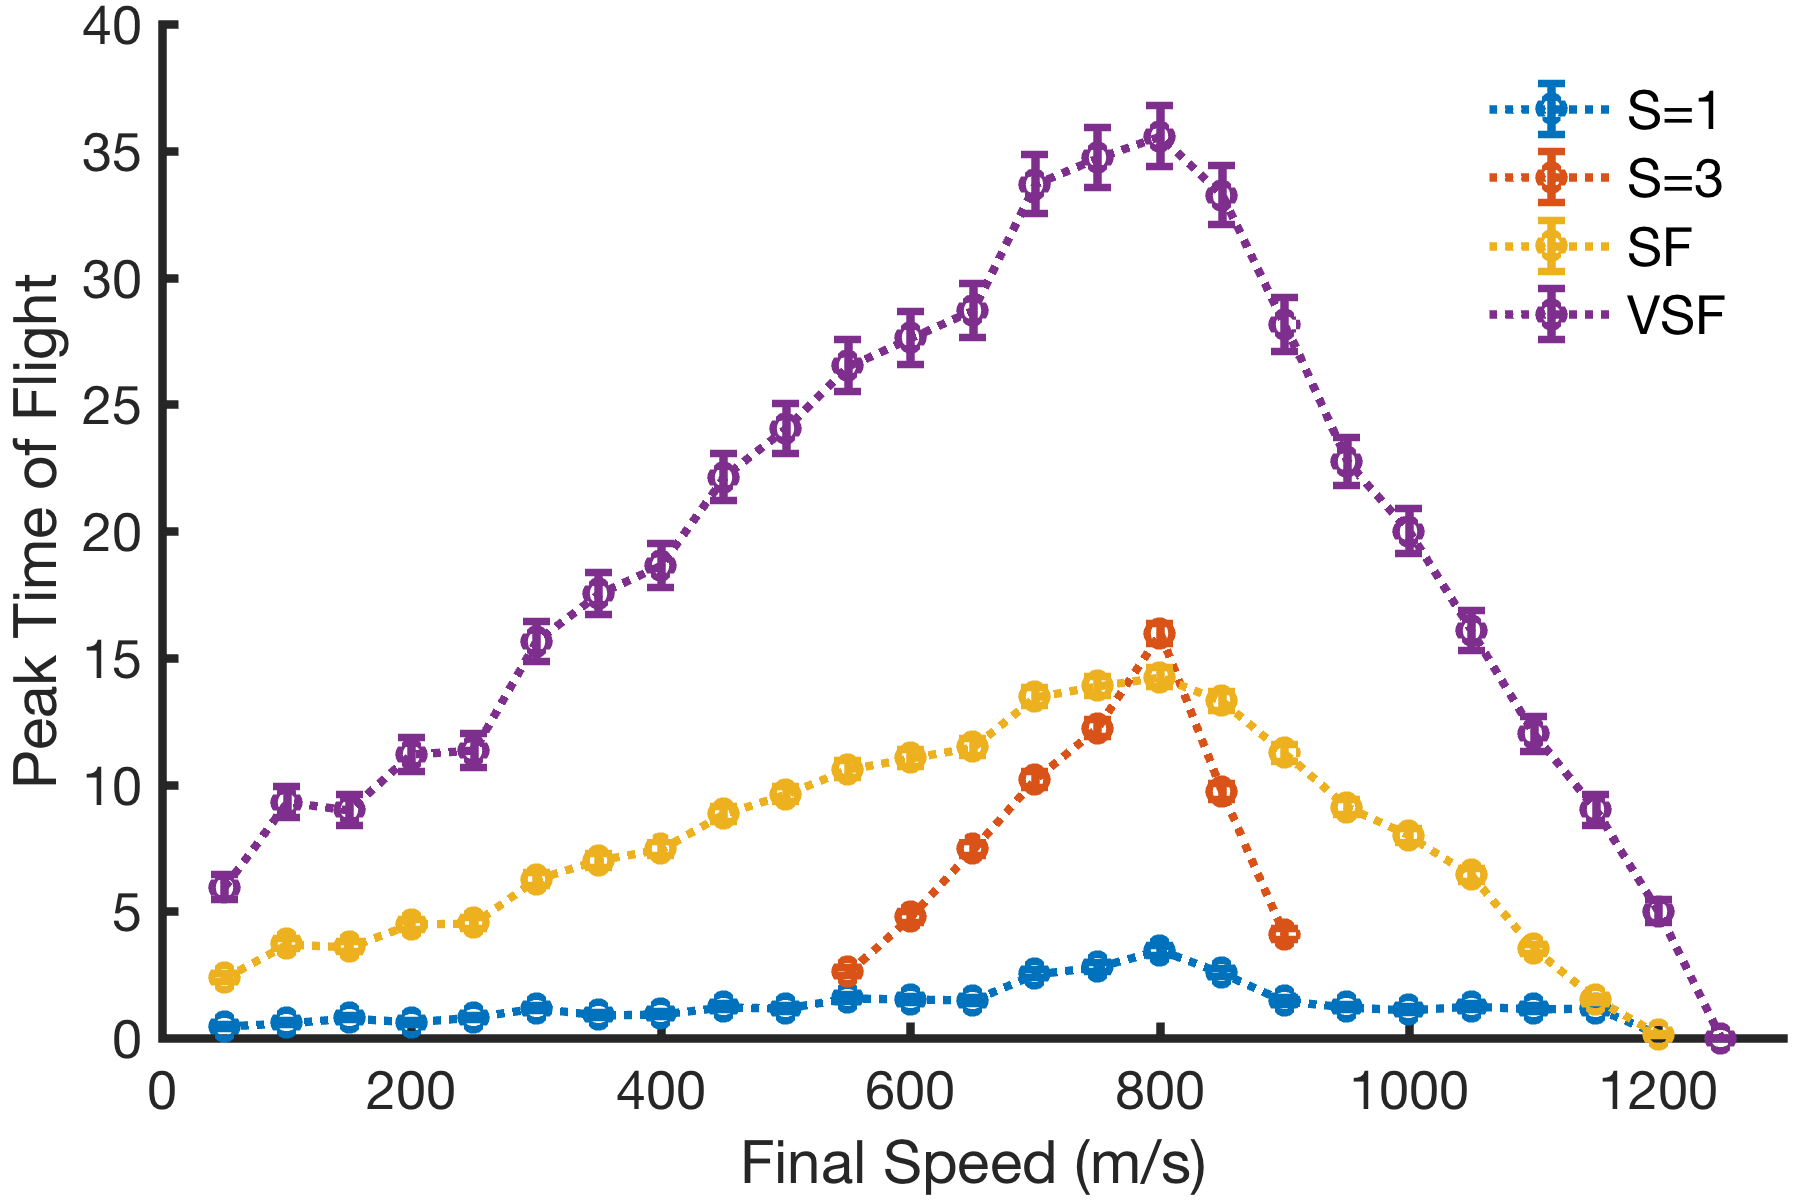
\includegraphics[width=\linewidth]{Data/Data-Figure-Final-Speed.png}%
\vspace{-5pt}
\caption{\label{fig:alldata}
Experimental comparison of deceleration strategies. 
Data are collected with a $333$ stage decelerator and a beam of OH radicals expanded in Neon at an initial speed of $820\text{ m/s}$. 
Large gains persist at low speeds, with F, an operating mode employing the new strategy, outperforming S\,=\,1 at $25\text{ m/s}$ sixfold.
\vspace{-4mm}
}
\end{figure}


The strategy is to admix new field distributions into the deceleration process that feature strong restoring force in the transverse directions.
%Field distributions with this property include those arising from applying voltage $V$ to only one of the four distribution rods in a Stark decelerator, from applying the same voltage $V$ to both pins in a pair rather than opposite polarities, 
Depending on which field distributions are admixed, we specify several operating modes employing this strategy: focusing (F), strong focusing (SF), and very strong focusing (VSF).
In the conventional strategy, only two field distributions are used, and one is identical to the other up to translation.
Operation modes employing the conventional strategy (S\,=\,1, S\,=\,3) vary only in the timing of switches between these distributions.
The measured performance of modes employing both strategies is shown in Fig.~\ref{fig:alldata} for hydroxyl radicals, a benchmark species for Stark deceleration.
These are performed on a decelerator not previously reported, with $2$~mm pin spacing and other geometric parameters as in our earlier devices~\cite{Bochinski2004,Sawyer2007}, but with more than double the length, $333$ stages, so as to decelerate a beam seeded in neon to rest.
F mode, which requires no wiring changes and may be immediately employed on existing devices, enhances performance by a factor of $4-8$ depending on final speed, see Fig.~\ref{fig:alldata}.
\begin{figure*}[t!]
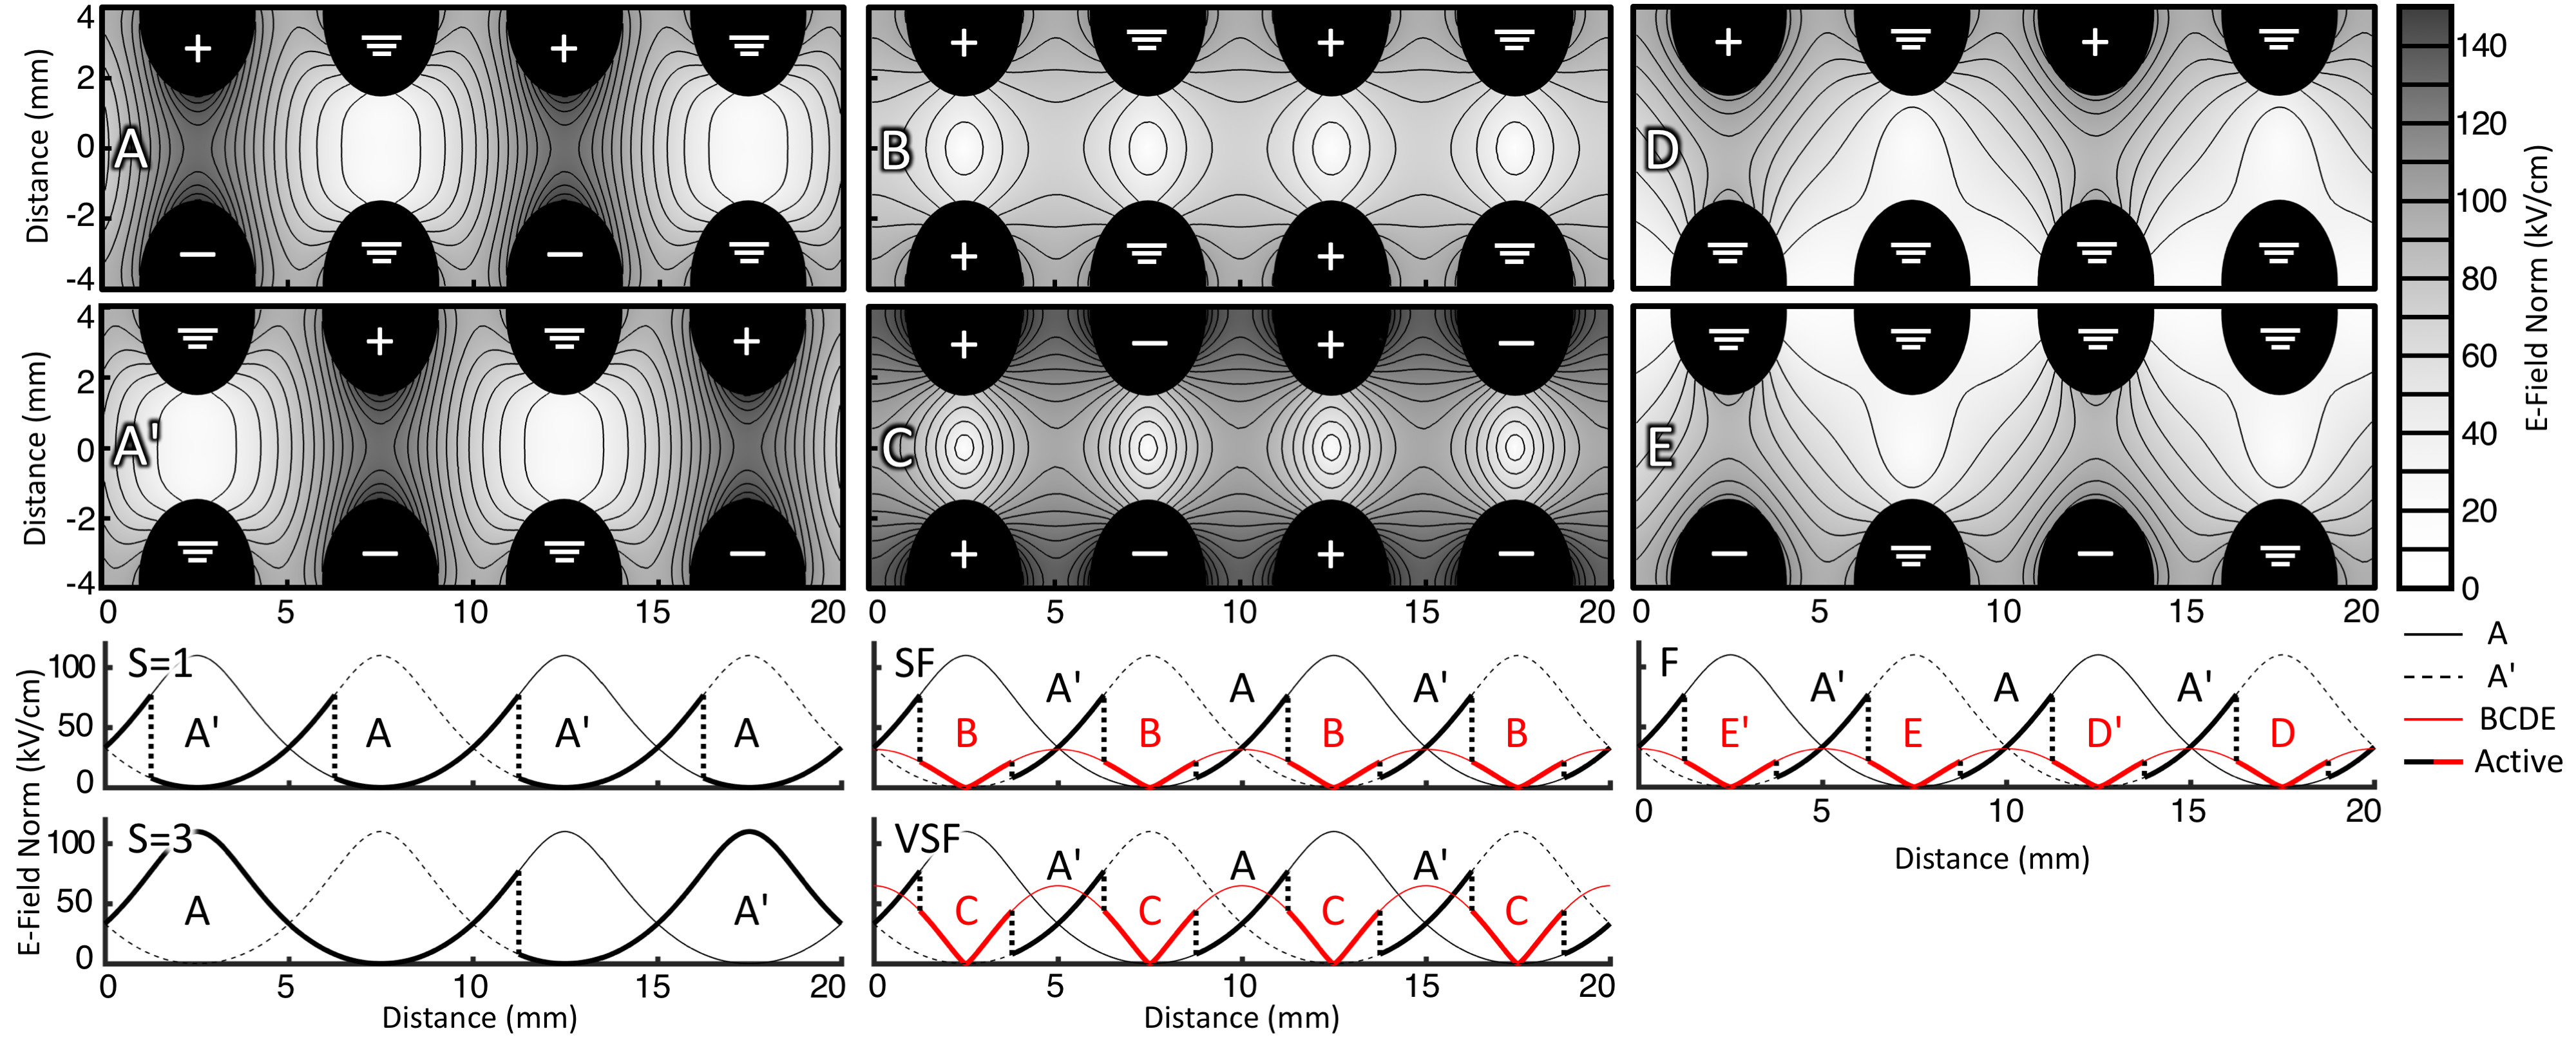
\includegraphics[width=\linewidth]{Configurations/pinpairformal6.png}%
\caption{
A new strategy for Stark deceleration, consisting of novel distributions of the electric field and operation modes which employ them. 
Upper left: the conventional distribution (A) and its translation to the next pin pair (A'). 
Upper right: distributions featuring enhanced transverse focusing (B--E). 
Below: On-axis energy diagrams for conventional operation modes S\,=\,1,3~\cite{VanDeMeerakker2005a}; and new operation modes named focusing (F), strong focusing (SF), and very strong focusing (VSF). 
These incorporate distributions D/E, B, and C respectively.  
Modes are aligned with the distributions they employ. 
Distributions are generated in COMSOL with $\pm12.5$~kV applied; the chosen cut plane includes the decelerator axis and is $45^\circ$ to all pins to ensure their visibility.
In this plane, distributions B and C show clear focusing between grounded pin pairs, and D/E work together to focus.
Distribution A seems field free between grounded pins, but in the plane orthogonal to the grounded pins it is in fact defocusing, as evidenced by the traveling potential well generated by S\,=\,1 mode in Fig.~\ref{fig:efftrap}. \vspace{-4mm}
}
\label{fig:chargecartoon}
\end{figure*}
Modes SF and VSF are not implemented in this work, but could be achieved with a new high voltage system for additional significant enhancement factors according to our simulations, see Fig.~\ref{fig:efftrap}.
%With some investment in high voltage equipment, it may be possible to implement SF mode, providing an additional significant gain even at trappable speeds. %which requires a tri-state switch capable of double the usual switching frequency~\footnote{Behlke HTS-301-151-SiC, options HFB, ILC, ALL-OFF-BIPOLAR.}, so as to make use of the field distribution arising from charging both pins in a pair to the same nenzero voltage.
%A comparable investment would enable VSF mode, but we do not pursue this since it is less useful for trapping, our primary emphasis, for reasons discussed below.
%The slowest speeds shown are suitable for trap loading~\cite{Sawyer2008}.
%Hold times vary from $2-4\text{ ms}$ as final speed is tuned, and thus are in agreement with the simulation results reported for $3\text{ ms}$ in Fig.~\ref{fig:efftrap}.

To understand the success of this new strategy, we revisit the operating principle of a decelerator; Fig.~\ref{fig:chargecartoon} details field distributions and the operating modes derived from them.
In the conventional strategy~\cite{VanDeMeerakker2012}, molecules approach a charged pin pair, climbing a hill in potential energy (Fig.~\ref{fig:chargecartoon}, left column). 
The hill is abruptly switched off, allowing molecules to then repeat the process without regaining that potential energy.
The abrupt switch occurs partway up the potential energy hill, so that molecules that are ahead get more energy removed, and vice versa. 
This creates a longitudinal restoring force for the molecules, with respect to the center of a decelerating reference frame.
It is customary to imagine an idealized ``synchronous molecule'' sitting in the center of this frame.
%This creates a traveling potential well for the molecules, with a longitudinal restoring force towards the center of a decelerating reference frame whose deceleration is set by the chirp rate of the switching frequency.
%It is customary to define an idealized ``synchronous molecule'' with zero energy with respect to this potential well, which proceeds exactly down the central axis of the decelerator and climbs each potential hill to the same position at the moment of a switching event.
In the transverse directions, restoring force is not inherited from switching events, but arises directly from the focusing properties of field distributions in the lab frame.
Together, the longitudinal and transverse restoring force generate a traveling potential well for the molecules, which translates along the device and decelerates according to a programmed ramp of the switching frequency.

Conventionally, pins are always charged in bipolar pairs, in which case transverse focusing occurs right between the charged pin pair, but not significantly elsewhere (Fig.~\ref{fig:chargecartoon}A).
This causes molecules to experience much better transverse focusing when they are regularly sampling the focusing fields right between the charged pin-pair, which requires them to be oscillating regularly ahead and behind the synchronous molecule.
Just after the switching event, which as mentioned must happen only partway up the potential energy hill, molecules proceed through the largely field-free region between grounded pin pairs.
This region is of central importance to our new deceleration strategy.
Useful field distributions with transverse focusing in this region can be created by applying voltage in a way that is not balanced between adjacent pin pairs. 
This imbalance causes field lines to run toward the grounded pin pair, creating a focusing 2D quadrupole structure, much like this one used intentionally for trapping and controlling spin-flip losses~\cite{Reens2017}.
Imbalanced distributions include those arising from charging only a single rod (Fig.~\ref{fig:chargecartoon}DE), from charging a pin pair to the same voltage (Fig.~\ref{fig:chargecartoon}B), or from charging the other pin pair oppositely (Fig.~\ref{fig:chargecartoon}C).
These correspond to modes F, SF, and VSF respectively.
By implementing these distributions when the synchronous molecule is flying between the grounded pin pair, but retaining the use of the conventional distribution otherwise (Fig.~\ref{fig:chargecartoon}, upper--lower alignment), the longitudinal behavior of the device is preserved while the transverse behavior is vastly improved.
%Refer to the on-axis energy diagrams in the lower half of Fig.~\ref{fig:chargecartoon}, and their alignment with the field distributions shown above them.

\begin{figure*}[ht!]
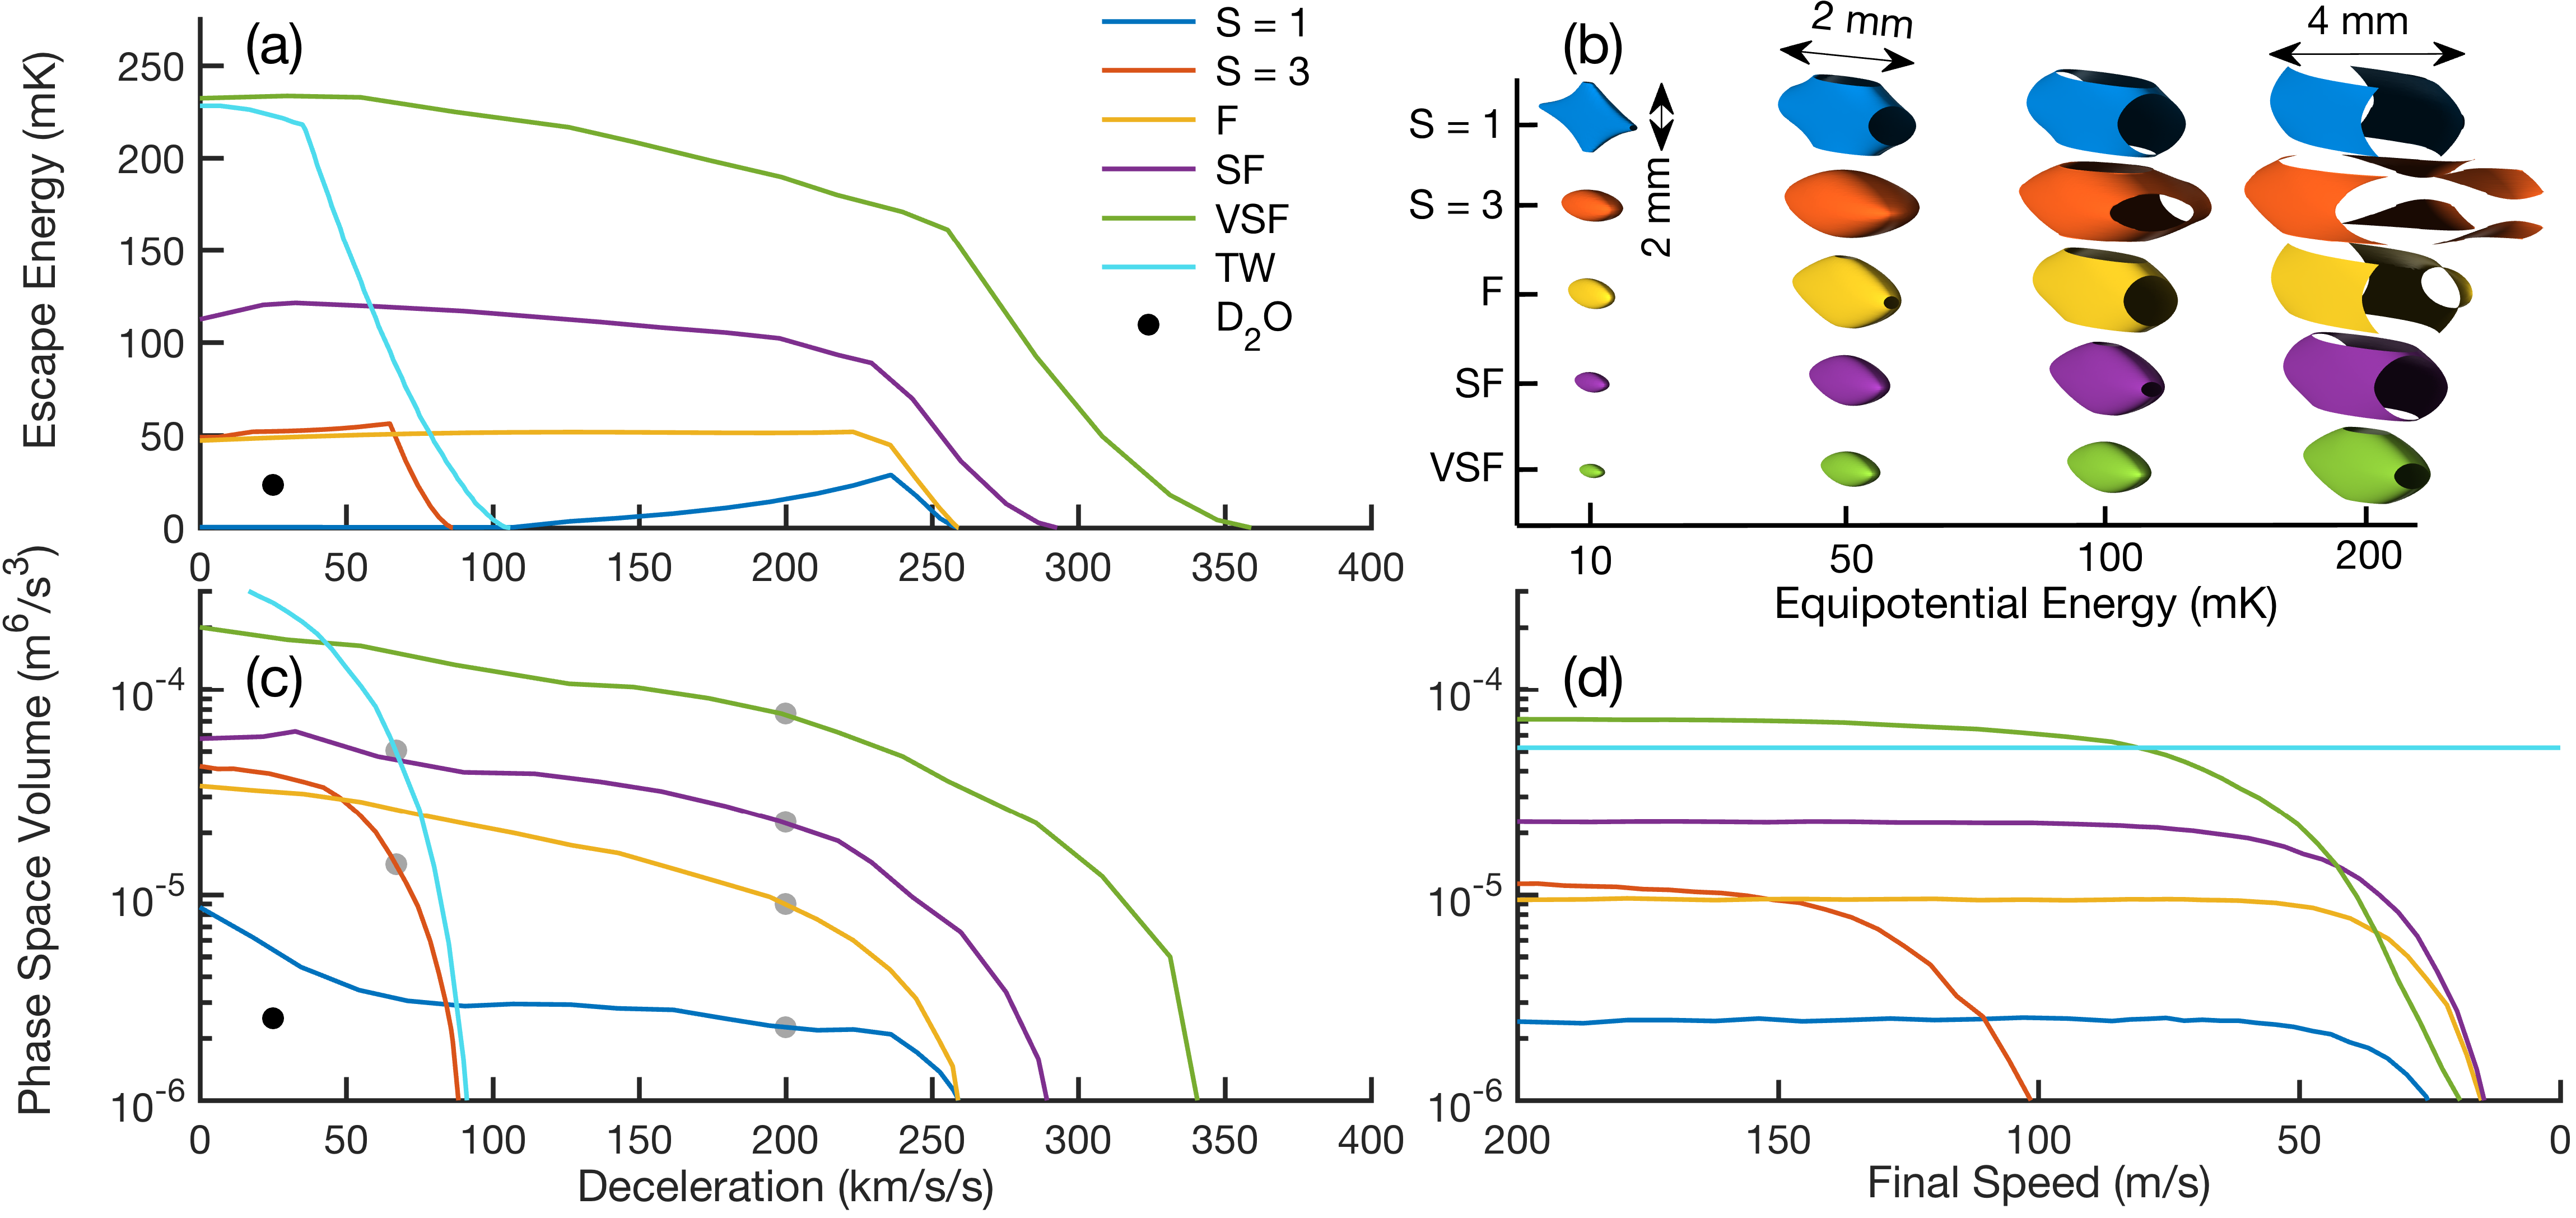
\includegraphics[width=\linewidth]{full-four-panel.png}%
\vspace{-5pt}
\caption{
Escape energy $E_\text{esc}$ from the traveling potential well generated by different modes of operation, for varying deceleration rate.
%Conventional S\,=\,1 and S\,=\,3 modes, together with F, SF, and VSF employing the new strategy. 
Traveling wave (TW) deceleration is also compared, assuming a $10$~kV peak to peak waveform. 
(a) $E_\text{esc}$ verse deceleration. A point is shown for heavy water~\cite{Motsch2009}.
(b) Equipotentials of the traveling well for $200$~km/s/s deceleration, or $67$~km/s/s for S\,=\,3 since this mode requires a triple length device.
Lack of closure of an equipotential equates to possibility of escape. 
(c) Initial phase space volume remaining within the traveling well after $3$~ms, only the effective traveling well is simulated. 
(d) Full decelerator simulation, agreeing with (c) at high enough final speeds, studied with varying final velocity but with hold time fixed at $3$~ms and deceleration fixed as indicated by the gray dots in panel~(c).
For TW a full simulation is not performed; the value corresponding to the dot in panel (c) is shown for comparison.\vspace{-4mm}}
\label{fig:efftrap}
\end{figure*}
%We identify several operational modes employing this strategy, varying according to the magnitude of their transverse focusing effects.
%Utilizing the field distribution arising from charging only a single rod, something readily achievable with no change to high voltage electronics, gives rise to F mode.
%Charging two pins to the same voltage gives rise to SF, and charging all four pins, one pair at one voltage and the next pair at the opposite voltage, gives VSF.

%\section{The Effective Moving Trap}
In order to quantitatively analyze these operation modes, we can directly calculate the traveling potential well they generate for the molecules.
This is performed as in~\cite{Bethlem2000,Hudson2004} but extended to three dimensions~\cite{ssm}.
The resulting wells may be visually inspected by plotting equipotential surfaces at various energies relative to the well minimum, see Fig.~\ref{fig:efftrap}b.
%These are calculated as described here~\cite{ssm}, where the same treatment as in~\cite{Bethlem2000,Hudson2004} is performed but with extension to three dimensions.
At some minimum escape energy $E_\text{esc}$, the traveling well equipotential fails to be closed, enabling molecules with energy $E\ge E_\text{esc}$ to escape. 
This escape may occur transversely, after which molecules encounter the surfaces of decelerator pins and are lost, or longitudinally, where molecules are not immediately lost but cease to remain in close proximity to the synchronous molecule.
$E_\text{esc}$ is plotted for all modes and as a function of varying decelerations in Fig.~\ref{fig:efftrap}a.
$E_\text{esc}$ is a useful figure of merit for characterizing the performance of a given operating mode, as evidenced by the close agreement between Fig.~\ref{fig:efftrap}a and Fig.~\ref{fig:efftrap}c, where the volume of initial phase space which will remain in the traveling well after a $3$~ms hold time is reported.

For the S\,=\,1 mode, $E_\text{esc}$ is nearly zero, particularly for molecules which move away from the trap center towards the four small escape holes barely visible in the $10$~mK S\,=\,1 equipotential of Fig.~\ref{fig:efftrap}b. 
This is the underlying reason for the transverse-longitudinal coupling problem that has been described~\cite{VanDeMeerakker2006}.
In general, such couplings are often useful for maintaining ergodicity in a potential well~\cite{Surkov1996}, but with some directions featuring very low escape energy, even small amounts of motional coupling lead to loss.
$E_\text{esc}$ actually improves with stronger deceleration for S\,=\,1, as expected given the increased sampling of the transversely focusing region when molecules climb further towards the charged pin pair, see Fig.~\ref{fig:chargecartoon}A.
Remarkably, F mode offers comparable $E_\text{esc}$ to S\,=\,3, but with no sacrifice in deceleration capability.
The SF and VSF modes make more dramatic improvements, with the latter rivaling traveling wave (TW) deceleration~\cite{Osterwalder2010}. 
In Fig.~\ref{fig:efftrap}, $10$~kV peak to peak sine waves are assumed, to our knowledge the largest used to decelerate all the way to rest~\cite{Quintero-Perez2013}.
Additionally, all modes besides TW use the rather small $2$x$2\text{ mm}^2$ open area of our device, while TW devices use rings of $4$~mm inner diameter.
If VSF mode were used with a $3$x$3\text{ mm}^2$ device~\cite{Scharfenberg2009} or a $4$x$4\text{ mm}^2$~\cite{VandeMeerakker2005}, phase space volume would increase significantly, depending approximately on the cube of pin-pair spacing. 

The domain of validity of the use of traveling wells to characterize deceleration is a key concern.
More commonly the traveling well approach is reserved for continuous deceleration schemes~\cite{Osterwalder2010,Narevicius2008}.
Essentially it is required that the longitudinal velocity $v_z$ of the molecules satisfy $v_z/D \gg f$, $D$ the stage distance and $f$ the oscillation frequency in the traveling well.
The precise dynamics as one approaches this bound are relevant, especially for trapping experiments, which necessarily violate this condition as $v_z\rightarrow 0$.
These dynamics may be precisely isolated by comparing the simulation of molecules in the traveling well (Fig.~\ref{fig:efftrap}c) to full Monte-Carlo simulations.
By varying only the final speed, and keeping deceleration and run-time exactly fixed by appropriately varying initial speed and decelerator length, we obtain the results shown in Fig.~\ref{fig:efftrap}d.
The asymptotically flat profiles at high enough speeds validate the traveling well approach, as do the quantitative agreement between the asymptotic values and the corresponding points at $200\text{ km/s/s}$ and $67\text{ km/s/s}$ in Fig.~\ref{fig:efftrap}c.

The beginning of the low-speed breakdown depends on the intended use of the decelerator, and especially how far the molecules will be expected to travel unguided afterwards.
In Fig.~\ref{fig:efftrap}c, the molecules still confined within a $3\text{ mm}$ diameter circle transversely after $5\text{ mm}$ free flight from the end of the sequence are shown. 
This is a conservative representation of what is required for trap-loading, but for collisional experiments a larger flight distance may be required.
Note how F and SF cut off at even lower speeds than S\,=\,1, but VSF cuts higher. 
This can be attributed to the fact that VSF actually features an increased transverse trap frequency relative to the others, while F and SF improve over S\,=\,1 mostly by mitigation of escape minima, and not by increasing the transverse confinement strength of the well.
VSF mode may be especially useful for trap loading in combination with a TW device as in~\cite{Quintero-Perez2013}.

%\section{Further Simulation Results}
\begin{figure}[t]
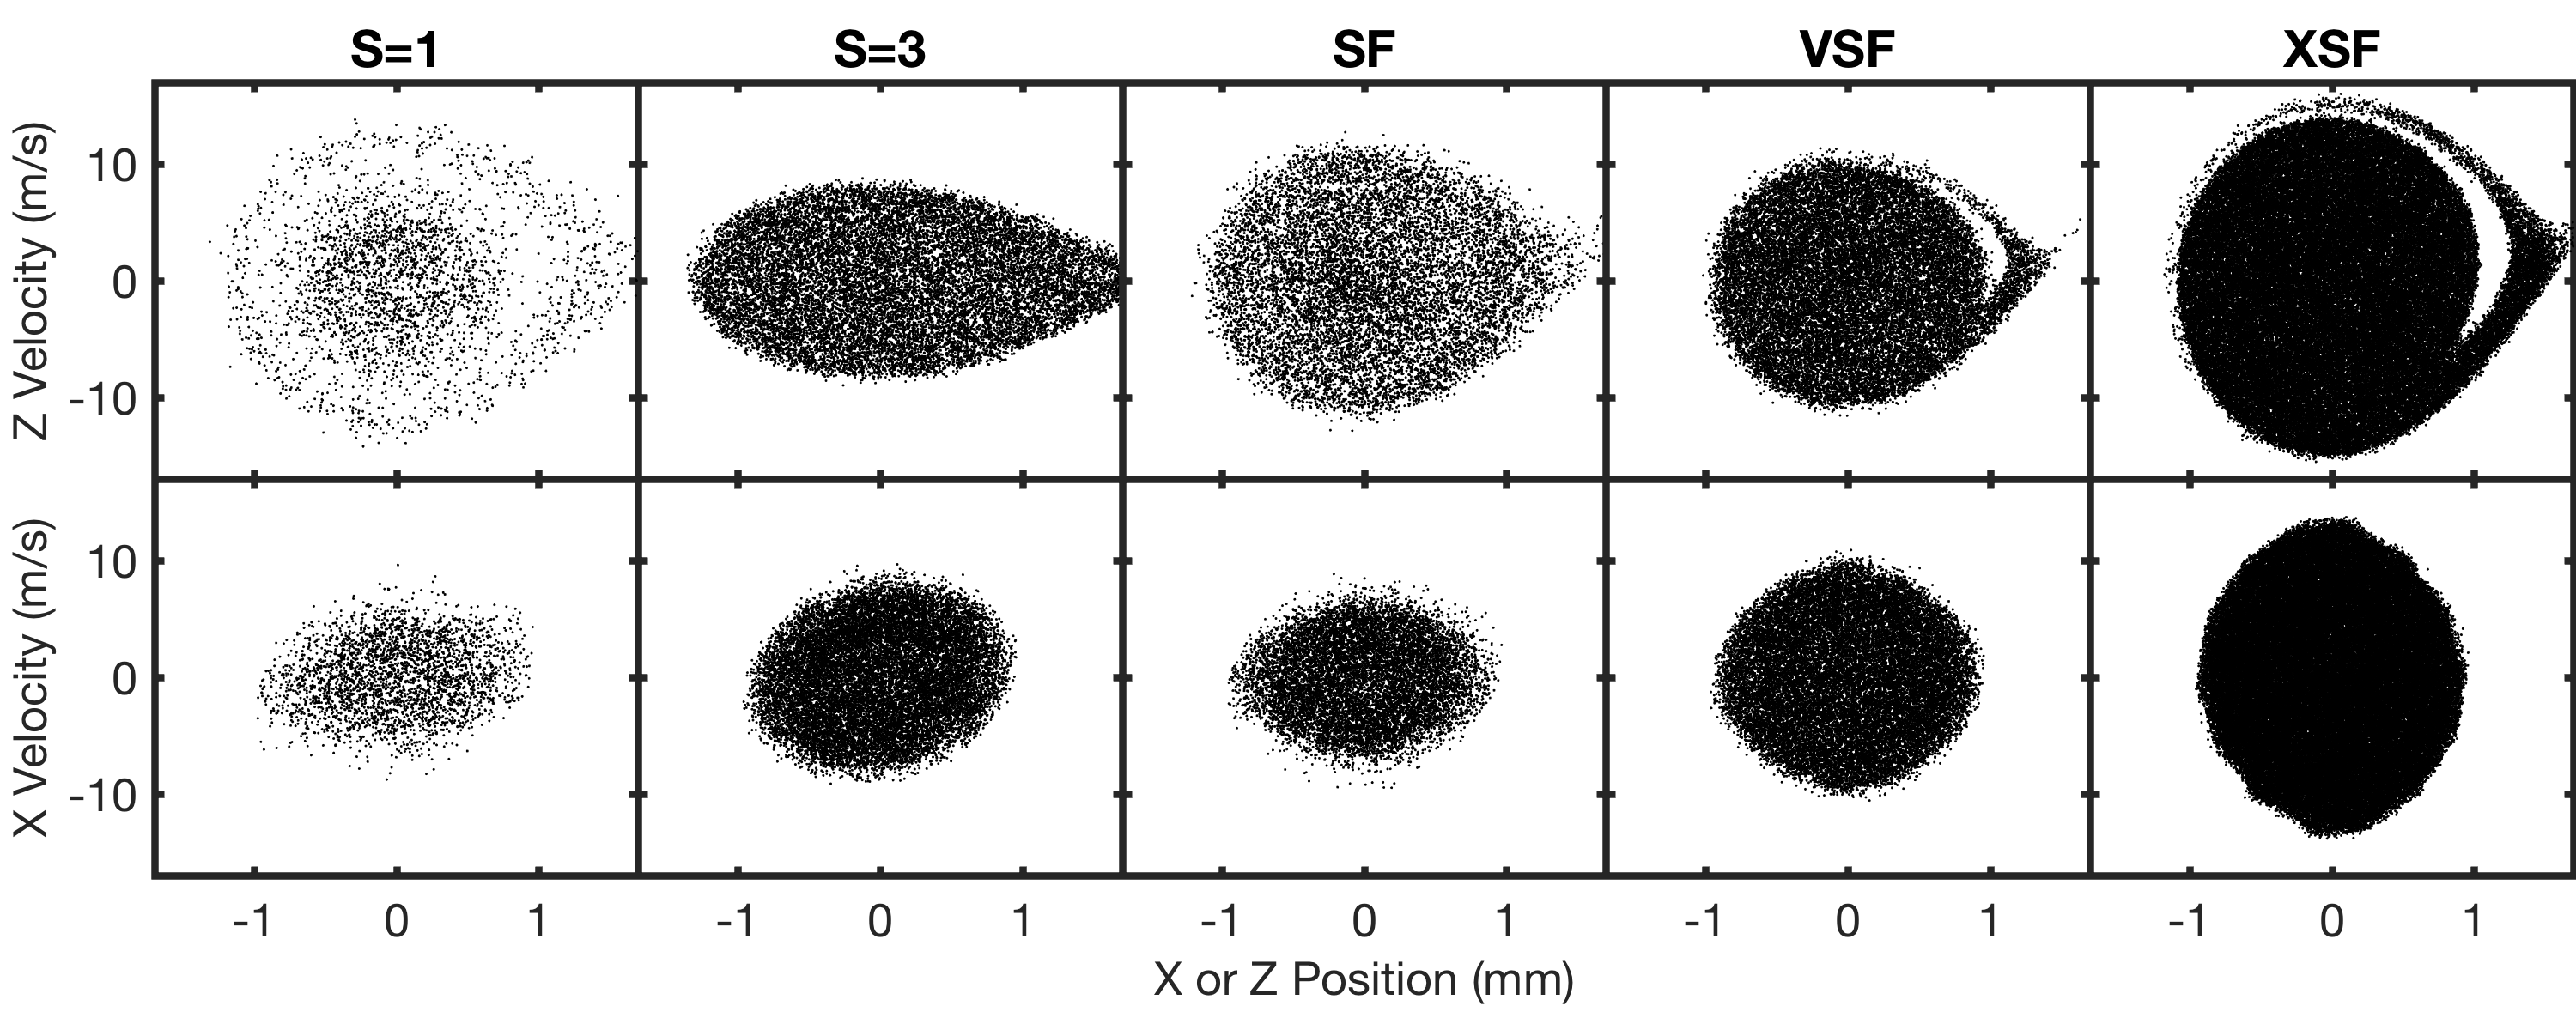
\includegraphics[width=\linewidth]{5x2-PSD-Compare.png}
\vspace{-15pt}
\caption{\label{fig:phasespace}
Phase Space Fillings, both longitudinal (above) and transverse (below), for the labeled operation modes. 
With the same uniformly distributed initial phase space, the surviving number of molecules is $3$, $17$, $11$, $24$, and $75$ thousand respectively.
Note dramatic improvements in homogeneity and flux, without significant broadening to larger velocity classes except for VSF. 
Molecules travel $333$~stages, begin at $900$~m/s, and slow at $200$~km/s/s ($67$~km/s/s for S\,=\,3), large decelerations useful for trap loading.
\vspace{-15pt}}
\end{figure}

In Fig.~\ref{fig:phasespace}, the longitudinal and transverse phase space fillings are compared for all modes, with $200\text{ km/s/s}$ deceleration through our $333$ stage device, and final speeds of about $200\text{ m/s}$ to avoid low speed cutoff behavior. 
All modes are initialized with the same homogeneous phase space density (PSD).
As can be seen, the distribution is nearly homogeneous after deceleration for all modes except S\,=\,1.
Increases in point density between panels do not arise from actual PSD increases, but from increases in the phase space volume that is projected onto the plane.
Nevertheless, these improvements can prevent reductions in PSD which stem from under filling of the phase space volume that a trap can accept.
For example, a hypothetical trap with an acceptance comparable to the outer dimensions of S\,=\,1 mode will be under filled by S\,=\,1 deceleration due to the missing regions, while F mode will not do this, effectively quadrupling the phase space density loaded in the trap.
Most realistic traps possess comparable transverse and longitudinal phase space acceptances due to ergodicity, cross-dimensional couplings, or cross-dimensionally thermalizing collisions if nothing else.
In SF mode, transverse phase space acceptance is increased significantly over F mode, becoming comparable to the longitudinal, and avoiding transversely under filling realistic traps by an additional factor of two.

%When comparing S\,=\,1 to F, phase space density is increased in a global sense, since the overall shape of the phase space acceptances are similar but quadruple the molecules are present in F.
%Locally however, phase space density is not increased; in the close vicinity of any point included on these plots, a suitably small phase space volume may be found within which phase space density is equal to the initial phase space density, in keeping with the Louisville theorem.
%The reason that phase space may be conserved locally but not globally is that the accepted region in S\,=\,1 mode, whose traveling well features low escape energies, becomes hopelessly swirled about, so that any reasonably shaped global volume will contain accepted regions of fixed phase space density and rejected regions of zero phase space density.

The homogeneous initial phase space density used in Fig.~\ref{fig:phasespace} is valid when the initial beam source generates a much broader distribution in phase space than the volume accepted by the traveling potential well.
In the longitudinal direction, most supersonic expansions satisfy this, with the exception of those performed with Helium buffer gas, which can reach temperatures as low as $40\text{ mK}$ expanding from room temperature~\cite{Even2014}.
For this work, OH expands in neon and reaches a $300\text{ mK}$ longitudinal temperature~\cite{Wu2018}, equivalent to a velocity spread of $\pm17$~m/s.
In the transverse direction, source temperature is a more subtle phenomenon, and may be bimodal~\cite{Beijerinck1981}.
Furthermore, beam skimming and the resulting interference it causes often require increased distance between the source and the decelerator, resulting in a transversely under-filled traveling well.
Skimmer cooling addresses this~\cite{Wu2018}, and is therefore well suited for VSF mode.

Finally, we note that the enhanced applicability of deceleration to less responsive molecules.
D$_2$O molecules in the $|1,1\rangle$ state~\cite{Motsch2009} are brought into the viable range in VSF mode, note the point at $25$~km/s/s in Fig.~\ref{fig:efftrap}c.
This is discussed further here~\cite{ssm}.

%It is observed that SF and VSF mode feature a very close match between their longitudinal and transverse phase space acceptances.
%This is a consequence of the tuning of an extra parameter afforded by the new deceleration modes- the relative time devoted to the original field distributions (Fig.~\ref{fig:chargecartoon}, A, A') and those with increased transverse focusing (Fig.~\ref{fig:chargecartoon}, B--E).
%In all mode diagrams shown in Fig.~\ref{fig:chargecartoon}, new field distributions are applied over a spatial region that is exactly centered around the grounded pin pair.
%But if this restriction is lifted, a new tuning parameter arises, a second phase angle $\phi_2$ of sorts.
%In Fig.~\ref{fig:efftrap}, $\phi_2$ is tuned for SF and VSF so as to maximize the escape energy for each deceleration.
%These tuned versions are labeled as SF$^*$ and VSF$^*$, and the optimum $\phi_2$ are listed in~\cite{ssm}.
%This escape energy is usually maximized when the transverse and longitudinal depths are made comparable, since otherwise one direction is limiting, hence the similar shape of the transverse and longitudinal distributions.
%Tuning $\phi_2$ for maximum escape energy tends to optimize flux as well, but one could instead tune for a desired ratio of longitudinal to transverse spread as required for optimal collisional studies or phase space matching to a trap.



%We also study the behavior of molecules in their effective moving traps at long times, see Fig.~\ref{fig:longtimes}.
%This allows us to distinguish several effects. 
%The very long-time asymptotic trapped number is a direct reflection of the effective moving trap depth.
%The time-scale for approach to this asymptotic number is a measure of the ergodicity of the effective trap.
%It is seen that in S=1 mode nearly all are lost eventually, as expected.
%It is also seen that while traveling wave geometries sport increased trap-depths, their asymmetry and increased ergodicity relative to VSF mode makes the latter preferable for a wide range of run-times useful in typical experiments.


%\section{Discussion}
%It is important to reconcile our language thus far with the notion of the phase space conservative behavior of non-dissipative Hamiltonian systems such as Stark decelerators. While it is true in theory that such systems cannot compress or dilute phase space; in practice the conserved volume can become hopelessly swirled about, so that any reasonable scientific device, which typically accepts an approximately ellipsoidal phase space volume, inevitably includes a mixture of conserved and non-conserved volumes, so that the final phase space density can be severely diluted. Simply put, a trap with a hole in it is certainly a non-dissipative Hamiltonian system, but that doesn't prevent molecules falling out.

%\section{Non-Adiabatic Transitions}
%Non-adiabatic transitions are important in the context of these alternate deceleration modes, because the charge configurations used for boosting transverse confinement feature quadrupolar field arrangements with electric field minima and rapid field rotation close to those minima.
%This situation makes possible transitions that preserve parity but change the $m$ quantum number describing the alignment of the molecule with the field.
%Molecular states chosen for Stark deceleration typically feature total $J>1/2$, in which case there exist states with less than maximal $|m|$ to which transitions can occur resulting in dramatically reduced strength of Stark forces applied by the decelerator.
%For the case of OH Molecules, $J=3/2$, and estimations of the magnitude of spin-flip transitions suggest that it could be as large as a $50\%$ effect in our device. 
%However, in practice, deviations from the ideal geometry tend to greatly reduce the risk of spin-flip transitions, because for example slight nonzero angles between pins, or length differences, tend to cause the unintentional removal of electric field minima.
%In our device, we find no detectable influence of spin-flip losses, based on good agreement between data and Monte Carlo without including their effect.
%This could be ensured by intentionally unbalancing the lengths of pin-pairs, so that one pair has rods that are a few millimeters longer than the other. A $3$~mm imbalance would be sufficient to pull the electric field zero completely out of the flight path of the molecules. 

%\section{Extensions}
%Besides XSF mode, mentioned above, several other direct extensions of our results are worth mentioning. Firstly, at low phase angles, we note that it is in general not worth the effort to mix in configurations $A$ and $A'$ of Fig.~\ref{fig:chargecartoon}, and good results can be achieved with only ever having a single rod charged at a time as in SF Mode. In the case of VSF mode, one can quite efficiently run a decelerator at low phase angles with only a single HV switch, by switching between configuration $D$ and configuration $0$, where only a small orientation preserving voltage is applied.

%For those interested in extending results in the direction of VSF mode but without tri-polar switches, gains can be made by admixing the configuration with all four rods charged to their normal voltages, also discussed as $\text{S}=3^+$ mode in Ref.~\cite{HudsonThesis2006}. Switching between the XSF configuration and the configuration with all pins charged at their normal voltages could be achieved with only two HV switches, and also affords XSF-like performance.

%Even restricting attention to the SF and VSF modes discussed primarily in this work, there is the possibility of tuning when the alternate configurations are applied and for how long. 
%We have studied this to some extent and found that applying the alternate configurations symmetrically about the grounded pin pair worked within 10\% of the optimum we could obtain by more carefully studying the space of possible timings.
%In general however, one could imagine much more thoroughly studying the space of possibilities, and even introducing the possibility of using more than two different configurations within a single stage, as performed in Ref.~\cite{Zhang2016} but for the usual charge configurations.

%Finally, we add that it may even be that a brand new electrode configuration is more well-suited for capitalizing on the gains afforded by the use of alternate charge configurations. The obvious direction would be to keep the pulsed design but somehow curve or change the pin arrangement so that the alternate configurations would feature even better focusing, without too dramatically reducing the magnitude of the large electric field that can be applied within a single stage in the usual configuration.

%\section{Conclusion}
We introduce a new deceleration strategy, with several accompanying modes of operation for the conventional pulsed decelerator. 
Significant improvements in transverse focusing and overall performance are demonstrated.
The strategy does not simply increase the temperature of molecules which may be decelerated.
Instead, by increasing the minimum escape energy $E_\text{esc}$ from the traveling potential well, molecule flux is enhanced at the same temperatures as before.
This discovery opens up possibilities for applying Stark deceleration to faster beams or to molecules with less favorable Stark shift to mass ratio, since decelerator length may be extended without suffering from low $E_\text{esc}$ in the traveling well.


%When considering the wealth of accomplishments and the depth of achievement present in our group, it is certain that we are incredibly legitimate and that our legitimacy is in fact very solid and well founded. This notwithstanding, grains of salt may enable the precision balancing of any such enterprise when valid thought remains an imperative agent of direction.



%includes uncited bib entries
%\nocite{*}
\bibliographystyle{apsrev4-1_no_Arxiv}
\bibliography{allrefs}

%\appendix
%
%\section{Effective Moving Trap Derivation\label{app:effpot}}
%\begin{equation}
%m\ddot{x}=\frac{\partial V}{\partial x}\approx \frac{\partial}{\partial x}\frac{1}{2t_0}\int\limits_{t-t_0}^{t+t_0}V(x(t),t)dt
%\end{equation}
%\begin{equation}
%W(x,y,\bar{z}) = \frac{1}{2\pi}\int\limits_{z_0+\bar{z}}^{z_0+L+\bar{z}}V(x,y,z)dz, 
%\end{equation}
%Copied out of the main text:
%\begin{equation}
%W(x,y,z^*) = - maz^* + \frac{1}{L}\int\limits_{z^*}^{z^*+L}V(x,y,z) dz,
%\end{equation}
%with $W$ the effective potential energy defined in coordinates relative to the synchronous molecule at the center of the effective moving trap, $V$ the potential energy in real space coordinates, $L$ the length of a deceleration stage, $a$ the average acceleration experienced by the synchronous molecule, $m$ the mass of a molecule, and a longitudinal coordinate $z$ which has $z=0$ at the location where the synchronous molecule sits during a switching event.
%
%where $z$ points along the decelerator axis, $V$ is the lab-frame potential energy induced via the Stark effect on the molecule and applied during propagation of the synchronous molecule from position $z_0$ to $z_0+L$, and $\bar{z}$ is the non-inertial transform from the lab-frame: 
%\begin{equation}
%\bar{z} = z + v_0 t - \frac{1}{2}a t^2.
%\end{equation}
%
%\begin{multline}
%W(x,y,z^*) = - maz^* + 
%\frac{1}{L'}\!\!\int\limits_{z^*}^{z^*+L'}\!\!V'(x,y,z) dz \\
%+\frac{1}{L-L'}\!\!\int\limits_{z^*+L'}^{z^*+L}\!\!V(x,y,z) dz,\hspace{2cm}
%\end{multline}
%where $V'$ represents the lab-frame Stark potential induced by the alternative charge configuration, and $L'$ gives twice the distance required for the synchronous molecule to fly from its longitudinal position during a switch event, to the center of the approaching pin pair which would have been grounded under S=1 operation. This hardly changes the longitudinal behavior of the device, but adds significant transverse depth to the effective moving trap.
%

\end{document}
%
% ****** End of file MolecularMajoranaLoss.tex ******


%% FIGURES
%Figures:
%Final Speed Panel, Sim & Expt. Add acceleration? Include extra focusing?
%1D longitudinal potential, transverse spring constant?
%2D trap contours, lab frame. Do in COMSOL.
%2D trap contours, eff frame. Gotta be Matlab. Show pins somehow.
%Phase Space Acceptance. Consider James� density coloring technique. Plot density as a function of 6D ball of increasing radius.
%Timing Diagram. Good way to show different chargings.
%Stage Number Dependence. Necessary? Interesting. Chance to work in chaos theory.
%3D trap surfaces? Need to try it to see if it is worth it.
%Is average potential same as average force?
















